%%%%%%%%%%%%%%%%%%%%%%%%%%%%%%%%%%%%%%%%%%%%%%%%%%%%%%%%%%%%%%%%%
% Contents: The home chapter
% $Id: grisbi-manuel-home.tex, v 0.4 2002/10/27 Daniel Cartron
% $Id: grisbi-manuel-home.tex, v 0.5.0 2004/06/01 Loic Breilloux
% $Id: grisbi-manuel-home.tex, v 0.6.0 2011/11/17 Jean-Luc Duflot
% some of its content was in menus chapter:
% $Id: grisbi-manuel-menus.tex, v 0.5.0 2004/06/01 Loic Breilloux
% $Id: grisbi-manuel-home.tex, v 0.8.9 2012/04/27 Jean-Luc Duflot
% $Id: grisbi-manuel-home.tex, v 1.0 2014/02/12 Jean-Luc Duflot
%%%%%%%%%%%%%%%%%%%%%%%%%%%%%%%%%%%%%%%%%%%%%%%%%%%%%%%%%%%%%%%%%

\chapter{Entering Grisbi\label{entrance}}%Entrée dans Grisbi

\section{Selecting a file\label{select-file}}%Sélection d'un fichier

\vspacepdf{3mm}			% vertical space = 5 mm

When you launch the application, Grisbi displays a page allowing you to get started in different ways.%Au lancement de l'application, Grisbi affiche la page qui vous permet de démarrer de différentes manières.

\vspacepdf{3mm}			% espace: 5 mm

You can display the Grisbi window in \indexword{full screen}\index{display!full screen}\index{full screen!display} by pressing the function key \key{F11}, and go back using the same key.%Vous pouvez afficher la fenêtre de Grisbi en \indexword{plein écran}\index{affichage!plein écran}\index{plein écran!affichage} par la touche de fonction \key{F11}, et revenir en arrière par la même touche.			% "!" separates the term from the subterm of the index entry

\vspacepdf{3mm}			% espace: 5 mm

\begin{figure}[htbp]			% h=here, t=top, b=bottom, p=page of float to force the figure here, not in a next page.
	\begin{center}					% image centrée
		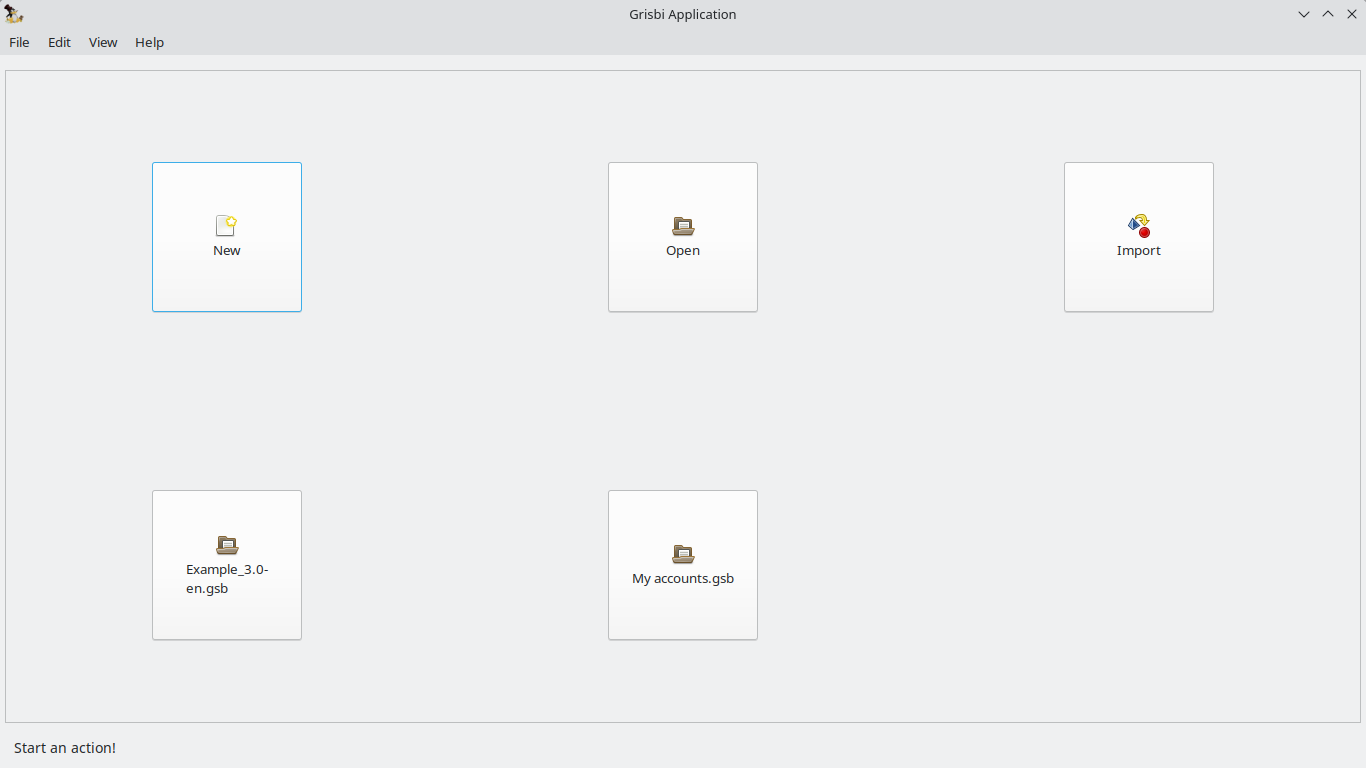
\includegraphics[width=0.95\textwidth]{image/screenshot/home_start_grisbi}		% width=95% as wide as the current text
	\end{center}
	\caption{Start-up window}%Fenêtre de démarrage}			% sous-titre/subtitle
	\label{home_start_grisbi}					% figure's ref., use for link in text with \refimage{}
\end{figure}

\vspacepdf{3mm}			% espace: 5 mm

In addition to the menu bar, this window displays a number of panels:%En plus de la barre de menu, cette fenêtre affiche plusieurs pavés:

\begin{itemize}
	\item the \enquote{New} button to launch the wizard \enquote{New file Assistant};%e pavé Nouveau, pour lancer l'assistant \frquote{Aide à la création d'un nouveau fichier de comptes};
	\item the \enquote{Open} button, to display a file manager that you can use to search for an existing accounts file on your computer;%le pavé Ouvrir, pour afficher un gestionnaire de fichier avec lequel vous pourrez chercher un fichier de comptes existant dans votre ordinateur;
	\item the \enquote{Import} button, to launch the \enquote{New file Assistant to import} wizard;%le pavé Importer, pour lancer l'assistant \enquote{Importation des opérations par Grisbi};
	\item one or more other buttons, named after account files Grisbi has already used.%un ou plusieurs autres pavés, portant le nom de fichiers de comptes que Grisbi a déjà utilisés.
\end{itemize}

\vspacepdf{5mm}	

\textbf{Note}: buttons with the names of account files that Grisbi has already used are only present if these files exist; if you want to remove them from this entry page, move them to another directory, or delete them.%les pavés portant les noms des fichiers de comptes que Grisbi a déjà utilisés ne sont présents que si ces fichiers existent; si vous voulez les enlever de cette page d'entrée, déplacez-les dans un autre répertoire, ou supprimez-les.

\vspacepdf{3mm}			% espace: 5 mm

At the bottom of the page, a banner invites you to choose an action by selecting one of these buttons.%En bas de page, un bandeau vous appelle à choisir une action en sélectionnant l'un de ces pavés.

\vspacepdf{3mm}			% espace: 5 mm

If you just want to discover the Grisbi software to get an idea of what it looks like and what it can do, you can instead use an example file like the one on the \lang{Sourceforge.net}\footnote{\urlSourceForgeDocumentation{}} site in the \enquote{\textsf{examples}} folder.%Si vous voulez juste découvrir le logiciel Grisbi pour avoir un aperçu de son aspect et de ses possibilités, vous pouvez à la place utiliser un fichier exemple comme celui présent sur le site de \lang{Sourceforge.net}\footnote{\urlSourceForgeDocumentation{}} dans le dossier \frquote{\textsf{examples}}.		% (voir la section \vref{new-example}).

\vspacepdf{5mm}			% espace: 5 mm

\textbf{Note}: by simply clicking on the downloaded example file, Grisbi will run, displaying the home window\refimage{home_3.0} directly without going through the start-up window.%en cliquant simplement sur le fichier exemple téléchargé, Grisbi s'exécutera en affichant directement la fenêtre d'accueil\refimage{home_3.0} sans passer par la fenêtre de démarrage.


\section{Homepage\label{home}}

\vspacepdf{3mm}

When an account file is opened, Grisbi displays its home page\refimage{home_3.0}.%When the application starts, Grisbi displays this
This is the start page of the programme and can be accessed at any time by clicking on the \menus{Accounts} tab.%This opening screen can be accessed at any time by clicking on the  \menus{Accounts} tab. 

\vspacepdf{3mm}

\begin{figure}[htbp]			% h=here, t=top, b=bottom, p=page of float to force the figure here, not in a next page.
	\begin{center}
		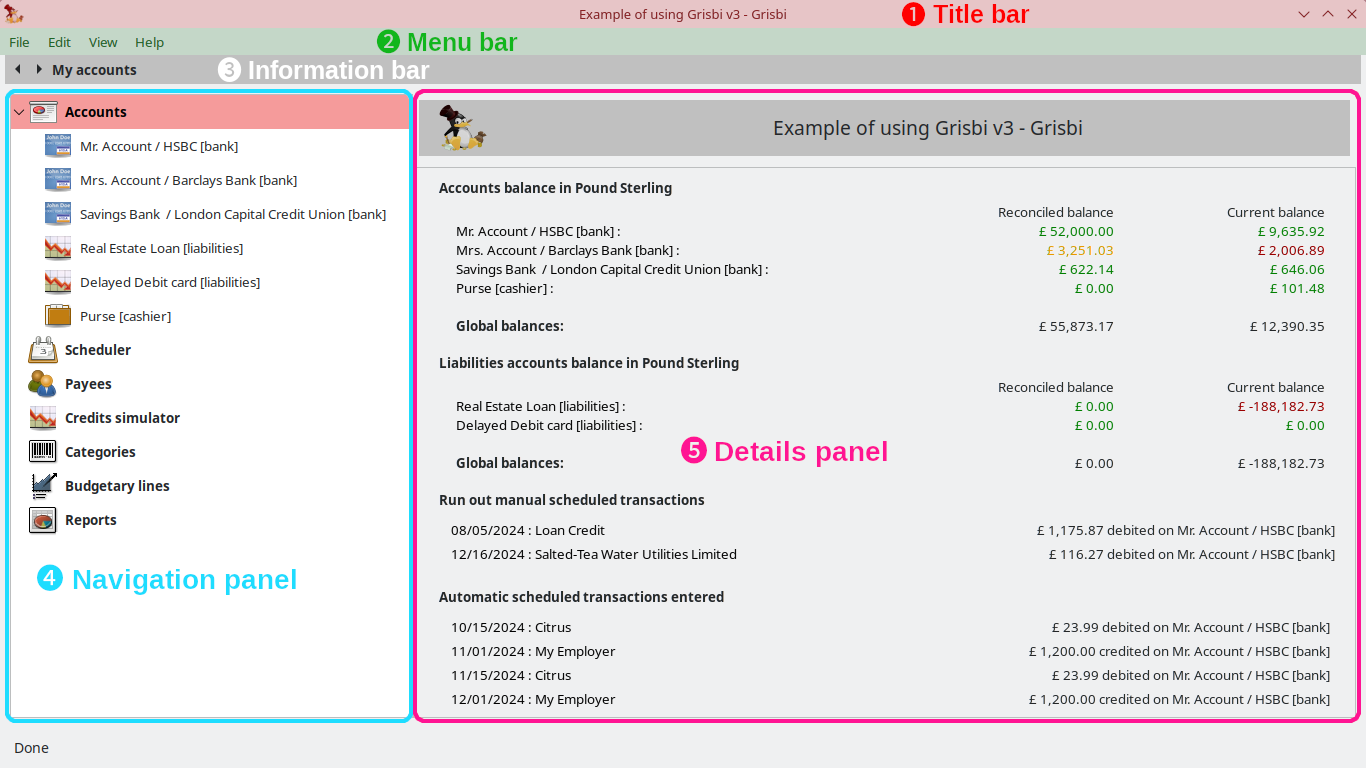
\includegraphics[width=1\textwidth]{image/screenshot/home_3.0.png}
	\end{center}
	\caption{Accounts summary page}		% sous-titre/subtitle
	\label{home_3.0}
\end{figure}

\vspacepdf{3mm}

Grisbi displays all pages in the same way: like any software, it displays:

\begin{itemize}%[\large \textcircled{\small 2}]
	\item[\large\textcircled{\small 1}] the title bar%une barre de titre;
	\item[\large\textcircled{\small 2}] the menu bar, which gives access to most of Grisbi's important functions;%une barre de menus qui donne accès à la plupart des fonctionnalités importantes de Grisbi;
\end{itemize}
as well as three specific Grisbi zones:%et aussi trois zones qui sont spécifiques à Grisbi:
\begin{itemize}%[3,4,5]
	\item[\large\textcircled{\small 3}] the information bar, under the menu bar;%la barre d'information, sous la barre de menus;
	\item[\large\textcircled{\small 4}] the navigation panel;%le panneau de navigation;
	\item[\large\textcircled{\small 5}] the details panel;le panneau des détails
\end{itemize}

\section{Information bar\label{home-synthesis}}

The information bar shows the name of the currently selected tab selected, and can display, completely to the right, certain balances relating to what is selected in the details panel.%The information bar shows the name of the current tab displayed, and can display, completely to the right, certain balances relating to what is selected in the details panel.%The information bar displays the name of the current tab displayed, and can display, to the far right, the current balance if one of the accounts is selected for display in the main screen area.

\vspacepdf{5mm}

\textbf{Note}: the information bar, displayed by default, can be hidden by unchecking a box in the preferences \vref{setup-display-toolbars}.

\vspacepdf{3mm}

To select one of the tabs displayed in the navigation panel click one or more times on one of the two small triangles on the top left of the panel.  The items displayed are: \menus{Accounts}, \menus{Scheduler}, \menus{Payees}, \menus{Credits simulator}, \menus{Categories}, \menus{Budgetary lines} and \menus{Reports}.  If the \menus{Accounts} and \menus{Reports} items have been expanded to display their sub categories these will also be displayed one by one.

\vspacepdf{5mm}

\textbf{Note}: Depending on the theme of the desktop environment or window manager you are using, these triangular symbols might be replaced by other characters such as +, -, >, <, etc.

\vspacepdf{3mm}
The content of the selection is displayed in the details panel.

\vspacepdf{3mm}
These functions can be used in place of the Navigation panel when its width is reduced to zero and you do not have direct access to it.


\section{Navigation panel\label{home-accounting}}

\begin{wrapfigure}{l}{0.33\textwidth}%50mm}
\vspace{-\intextsep}				% space above the floating (minus intextsep=separation between float and text in text)
\centering							% centering the floating figure in the "wrap"
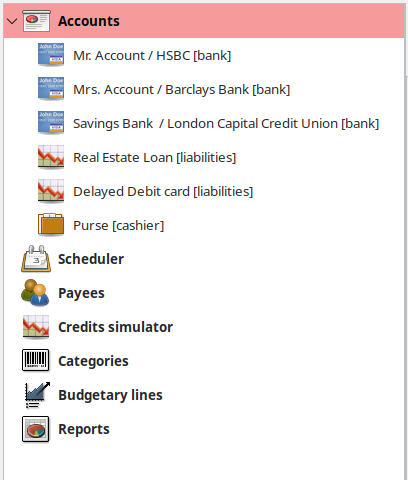
\includegraphics[width=0.28\textwidth]{image/screenshot/home_navigation}
\vspace{-5pt}						% space between the floating and the caption below the floating
\captionsetup{%						% for a change of options of the caption package
	format=plain,					% to avoid error message with labelsep option below, default=hang
	name=Fig.,						% rename label caption, default="Figure" (or "Table")
	justification=centering,		% centring of text and caption label 
	labelsep=newline				% define the separator between the label and the caption text
}
\caption{Navigation panel}		% \caption is mandatory to reference a figure in lof
\vspace{-40pt}						% space below the caption
\label{home_navigation}
\end{wrapfigure}

The navigation panel displays in bold the list of tabs:
	\begin{itemize}
		\item \menus{Accounts},
		\item \menus{Scheduler},
		\item \menus{Payees},
		\item \menus{Credits simulator},
		\item \menus{Categories},
		\item \menus{Budgetary lines},
		\item \menus{Reports}.
	\end{itemize}
By clicking on the small black triangle to the left of the \menus{Accounts} or \menus{Reports} tabs,  you can scroll or roll up the list of their sub-tabs. You can change the order of tabs and sub-tabs by clicking on one of them and dragging it up or down the list.

\vspacepdf{5mm}

\textbf{Note}: Depending on the theme of the desktop environment or window manager you are using, these triangular symbols might be replaced by other characters such as +, -, >, <, etc.

\vspacepdf{3mm}

You can select one of these tabs or sub-tabs by clicking on its name. You can also move the selection in this list of tabs and sub-tabs with the \keys{Up Arrow}, \keys{Down Arrow}, \keys{Page Up} ou \keys{Page Down} keys, or with the mouse wheel (option to be checked in the preferences \vref{setup-display-toolbars}). 

\vspacepdf{3mm}
The contents of the selection are displayed in the details panel.

\vspacepdf{3mm}
You can reduce or enlarge the width of the navigation panel by clicking on the thin vertical bar between this panel and the details panel, and moving it. If the width of the window has been reduced to zero, or enlarged to the maximum of the width of the Grisbi window, the thin vertical bar may be to the left or to the right of the window.  Locate this and slide it back to the desired location.

\vspacepdf{3mm}

The \indexword{context menus}\index{context menus}, accessible by a right-click of the mouse, are available on the elements of this panel and offer the following functions:

\begin{itemize}
	 \item On \menus{Accounts}:
		\begin{itemize}
			 \item \menus{New account};
		\end{itemize}
	 \item On any account: 
		\begin{itemize}
			 \item \menus{New account},
			 \item \menus{Remove this account};
		\end{itemize}
	 \item On \menus{Payees}:
		\begin{itemize}
			 \item \menus{New payee},
			 \item \menus{Delete selected payee},
			 \item \menus{Edit selected payee},
			 \item \menus{Manage payees},
			 \item \menus{Remove unused payees};
		\end{itemize}
	 \item On \menus{Categories}: 
		\begin{itemize}
			 \item \menus{New category},
			 \item \menus{Delete selected category},
			 \item \menus{Edit selected category},
			 \item \menus{Import a file of categories (.csgb)},
			 \item \menus{Export the list of categories (.csgb)}:
		\end{itemize}
	 \item On \menus{Budgetary lines}:
		\begin{itemize}
			 \item \menus{New budgetary line},
			 \item \menus{Delete selected budgetary line},
			 \item \menus{Edit selected budgetary line},
			 \item \menus{Import a file of budgetary lines (.isgb)},
			 \item \menus{Export the list of budgetary lines (.isgb)};
		\end{itemize}
	 \item On \menus{Report}: \menus{New report};
	 \item On any report: 
		\begin{itemize}
			 \item \menus{New report},
			 \item \menus{Remove this report}.
		\end{itemize}
\end{itemize}

\section{Details panel\label{home-details}}

The details panel displays all the details on the tabs or sub-tab selected by the Information bar or Navigation panel. This is the main work area of Grisbi.

You can reduce or enlarge its width by clicking on the thin vertical bar between this window and the navigation panel, and dragging it. If the width of the this panel has been reduced to zero or enlarged to the maximum of the width of the Grisbi window, the thin vertical bar may be to the left or to the right of the window. Locate this and slide it back to the desired location.

\begin{figure}[htbp]			% h=here, t=top, b=bottom, p=page of float to force the figure here, not in a next page.
	\begin{center}
		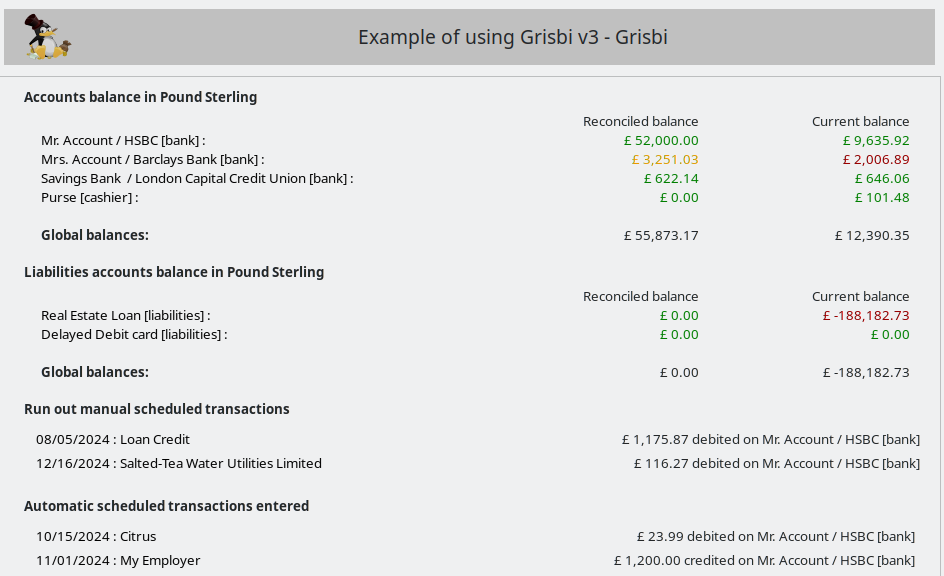
\includegraphics[width=1\textwidth]{image/screenshot/home_details.png}
	\end{center}
	\caption{Modified details panel}		% sous-titre/subtitle
	\label{home_details}
\end{figure}
 
\subsection{Displaying details on the home page\label{home-details-homepage}}

By selecting the \menus{Accounts} tab, the details panel displays:

\begin{itemize}
	\item to the top in a grey background banner:
		\begin{itemize}
			\item on the left, the \menus{Grisbi} icon (which can be hidden, see \vref{setup-display-logo-icon}),
			\item and on the right the \indexword{title}\index{title display!title}\index{home page} of the accounts file you currently have loaded, in the form \enquote{assigned name - Grisbi}; you can define this label, from among three possibilities, in the \menus{Edit - Preferences} menu (see the \vref{setup-display-addresses-titles} paragraph, Addresses \& titles):
				\begin{itemize}
					\item the \menus{Accounting entity} (by default): this is the name you use to identify the type of account e.g. \enquote{My Accounts} or \enquote{Business}, which you entered when the account file was created; you can edit it here in the \menus{Name of accounting entity} field; this can be useful if you manage multiple \indexword{accounting entities}\index{accounting entity}, 
					\item the \menus{Account owner name}: the name of the owner (or account manager) of the last account accessed; if the holder is not defined in the account properties, Grisbi displays the name of this account,
					\item the \menus{Filename}: this is the name of the file in the current directory, in the form  \file{name\_of\_your\_file.gsb};
				\end{itemize}
		\end{itemize}
	\item in the main light grey area below the banner:
		\begin{itemize}
			\item for each currency separately, for all accounts and \indexword{groups of accounts}\index{group of accounts}, under the label \menus{Reconciled balance} and \menus{Current balance}:
				\begin{itemize}
					\item the balance of the bank and cash accounts, the partial balance of the groups of accounts and their global balance,
					\newline
					\textbf{Note}: you can adjust the display order of the partial balances of the account groups (see the section \vref{setup-general-home-partBalance}, \menus{Partial balances of the list of accounts}),		 
					\item the balance of the liability accounts and their final balance,
					\item the balance of the asset accounts and their final balance;
				\end{itemize}
			\item the \indexword{warnings from automatically scheduled entries}\index{alert!scheduled entry} with their date, wording and amount, according to the choices made in the \menus{Edit - Preferences} menu (see the section \vref{setup-general-planned}, \menus{Scheduler}),
			\item the list of accounts whose balance has fallen below the \menus{Minimum authorized balance},
			\item the list of accounts whose balance has fallen below the \menus{Minimum desired balance}.
		\end{itemize}
\end{itemize}

\vspacepdf{5mm}

\textbf{Note}: For definitions of \menus{Minimum authorized balance} and \menus{Minimum desired balance}, see the \vref{accounts-properties}, \menus{Account Properties} section.

\vspacepdf{3mm}

The account labels are displayed in \textcolor{black}{black}: as the mouse cursor moves over the line of one of these, its colour changes to \textcolor{gray}{grey}.

A balance greater than the \menus{Minimum desired Balance} is displayed in \textcolor[RGB]{0,126,0}{green}: as the cursor moves over the line, its colour changes to \textcolor[RGB]{0,227,0}{light green}.

A balance less than the \menus{Minimum desired balance} and greater than the \menus{Minimum authorized balance} is displayed in \textcolor[RGB]{230,155,0}{orange}: as the pointer passes on its line, this color changes to \textcolor[RGB]{255,200,0}{light orange}.

A balance less than the  \menus{Minimum authorized Balance}  is displayed in \textcolor[RGB]{153,0,0}{dark red}: as the pointer passes over its line, this color changes to \textcolor{red}{red}.

When you move the mouse pointer over the line of an account, any color change indicates that if you click (right or left) with the mouse, the records contained in the highlighted account is displayed, as if the account had been selected with the information bar or navigation panel.

A partial balance can be specified for a group of accounts  If defined this is displayed in \textcolor[RGB]{40,40,255}{dark blue} (as in the figure \vref{home_details}). If it is negative, it may appear in \textcolor[RGB]{153,0,0}{dark red}, (see  \vref{setup-general-home-partBalance}, \menus{Balances partials of the list of accounts}). A partial balance line does not change color when the mouse pointer is over it, because you can not view the individual entries for of an group of accounts.

% espace pour changement de thème
\vspacepdf{3mm}
You can configure certain aspects of the display of the details panel:
\begin{itemize}
	\item in the \menus{Edit - Preferences} menu: %TODO verify sections/paragraphs with \vref{setup-xxx}
		\begin{itemize}
			\item \menus{\indexword{Generalities}\index{generalities}}:
				\begin{itemize}
					\item \menus{Various settings}, \menus{Scheduler}\index{scheduler} tab: section \vref{setup-general-planned};
					\item \menus{Main page}:
					\begin{itemize}
						\item \menus{Calculation of balance}: paragraph \vref{setup-general-home-balance},
						\item \menus{Balances partials of the list of accounts}: paragraph \vref{setup-general-home-partBalance};
					\end{itemize}
				\end{itemize}
			\item \menus{\indexword{Display}\index{display}}:
				\begin{itemize}
					\item \menus{Fonts \& Logo}\index{fonts}\index{logo}: section \vref{setup-display-logo},
					\item \menus{Addresses \& titles}\index{title}\index{addresses}: section \vref{setup-display-addresses-titles};
				\end{itemize}
	 	\end{itemize}
 	\item in the \menus{Properties} tab of each account in the \menus{Balances} section:
	 	\begin{itemize}
	 		\item Accounts below the \menus{Minimum authorised balance}\index{balance!minimum authorised}: section \vref{accounts-properties}:
	 		\item Accounts below the \menus{Minimum desired Balance}\index{balance!minimum desired}: section  \vref{accounts-properties}.
	 	\end{itemize}
\end{itemize}

%In particular, if you find a spelling error in this page, you can correct it: see the paragraph \vref{setup-general-home-final}, \menus{?? Pluriel de final ??} !

\section{Menu bar\label{home-menus}}

As in many graphics applications, most of Grisbi's important features are accessible through the menus in the \indexword{Menu Bar}\index{menu bar}. The features are detailed below.


\subsection{\menus{File} menu\label{home-menus-file}}

This menu includes the following functions:

\vspace{3mm}
\begin{itemize}[rightmargin=.6cm]
	\item \menus{New window}: non-functional (perhaps in the future?) %TODO: to update
\end{itemize}

\noindent
\begin{minipage}{.7\linewidth}
	\begin{itemize}[rightmargin=.6cm]
		\item \menus{New account file}: creates a new Grisbi file of \gls{extension}\file{.gsb}; the current file is therefore closed and a new empty file is created with an empty account (shortcut \keys{Ctrl+N}), see the section \vref{start-newfile}; not to be confused with the creation of a new account;%\menus{Nouveau fichier de comptes}: crée un nouveau fichier Grisbi d'\gls{extension} \file{.gsb}; le fichier courant est donc fermé et un nouveau fichier vide est créé avec un compte vide (raccourci-clavier \keys{Ctrl+N}), voir la section \vref{start-newfile}; à ne pas confondre avec la création d'un nouveau compte;	 
		\item \menus{Open}: opens your file manager, allowing you to search for, select and open an account file with the \file{.gsb} \gls{extension} (shortcut \keys{Ctrl+O}).%ouvre votre gestionnaire de fichiers, permettant de rechercher, sélectionner et ouvrir un fichier de comptes d'\gls{extension} \file{.gsb} (raccourci-clavier \keys{Ctrl+O});
		\item \menus{Recently opened files}: displays a list of the last n files opened with Grisbi (only if more than one has been opened); this number is configurable in the menu \menus{Edit - Preferences}, see section \vref{setup-general-files-manage}, \menus{Account Files Management};%affiche la liste des n derniers fichiers ouverts avec Grisbi (seulement s'il y en a eu plusieurs); ce nombre est configurable dans le menu \menus{Edition - Préférences}, voir la section \vref{setup-general-files-manage}, \menus{Gestion des fichiers de compte};
	\end{itemize}
\end{minipage}
\hspace{10pt}	
\begin{minipage}{.3\linewidth}
	\vspace{-10pt}					% space above the floating (minus intextsep=separation between float and text in text)
	\centering						% centering the floating figure in the "wrap"
	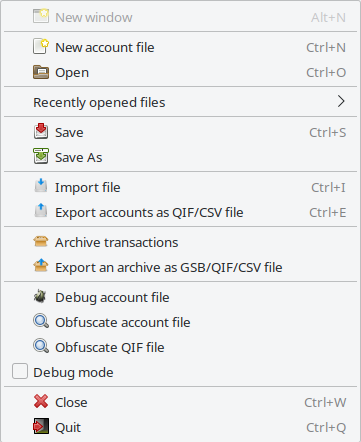
\includegraphics[width=1\textwidth]{image/screenshot/home_menubar_file}
	\vspace{-10pt}					% space between the floating and the caption below the floating
	\captionsetup{
		type=figure,%				% define "figure" or "table" type, mandatory
		name=Fig.,%					% rename label caption, default="Figure" (or "Table")
		labelsep=newline}			% define the separator between the label and the caption text
	\caption{\menus{File} menu}	% \caption is mandatory to reference a figure in lof
	%\vspace{30pt}					% space below the caption
	\label{home_menubar_file}
\end{minipage}

\begin{itemize}
	\item \menus{Save}: Saves the current account file (shortcut \keys{Ctrl+S});%\menus{Enregistrer}: enregistre le fichier de comptes en cours (raccourci-clavier \keys{Ctrl+S});
	\item \menus{Save As}: opens a file manager to save the current accounts file with the name and location of your choice; Grisbi defaults to the current directory, the name of the current accounts file, with the \file{.gsb} extension;%\menus{Enregistrer sous}: ouvre un gestionnaire de fichiers pour enregistrer le fichier de comptes en cours avec le nom et à l'emplacement de votre choix; Grisbi vous propose par défaut le répertoire courant, le nom du fichier de comptes en cours, avec l'\gls{extension} \file{.gsb};
	\item \menus{Import file}: starts the \enquote{Importing transactions into Grisbi} wizard of another software (shortcut \keys{Ctrl+I}); see \vref{move-import-importinit};%\menus{Importer un fichier}: démarre l'assistant d'importation de fichiers d'un autre logiciel (raccourci-clavier \keys{Ctrl+I}); voir la section \vref{move-import-importinit};
	\item \menus{Export accounts as \gls{QIF}/\gls{CSV} file}: starts the \enquote{Exporting Grisbi accounts} wizard (shortcut \keys{Ctrl+E}); see \vref{move-export};%\menus{Exporter vers un fichier QIF/CSV}: démarre l'assistant d'exportation de fichiers de compte (raccourci-clavier \keys{Ctrl+E}); voir la section \vref{move-export};	
	\item \menus{Archive transactions}: starts the archive creation wizard; see \vref{datamanagement-history-new};%\menus{Créer une archive}: démarre l'assistant de création d'archive; voir la section \vref{datamanagement-history-new};	
	\item \menus{Export an archive as \gls{GSB}/\gls{QIF}/\gls{CSV} file}: starts the archive export wizard; see \vref{datamanagement-history-export};%\menus{Exporter une archive vers un fichier GSB/QIF/CSV}: démarre l'assistant d'exportation d'archive; voir la section \vref{datamanagement-history-export};
	\item \menus{Debug account file}: starts the debug wizard for this file, which will help you look for inconsistencies in your account file; see \vref{maintenance-file-debug};%\menus{Déboguer le fichier de comptes}: démarre l'assistant de débogage de ce fichier, qui va vous aider à chercher des incohérences dans votre fichier de comptes; voir la section \vref{maintenance-file-debug};
	\item \menus{Obfuscate account file}: starts the wizard that produces an anonymous copy of your account file; this file can be attached to a bug report; see \vref{maintenance-file-anonymous};%\menus{Rendre anonyme le fichier de comptes}: démarre l'assistant qui produit une copie anonymée (de manière irréversible) de votre fichier de comptes; ce fichier pourra être joint à un rapport de bogue; voir la section \vref{maintenance-file-anonymous};	
	\item \menus{Obfuscate QIF file}: starts the wizard that produces an anonymous copy of this file; this file can be attached to a bug report; see \vref{maintenance-QIF-anonymous};%\menus{Rendre anonyme le fichier QIF}: démarre l'assistant qui produit une copie anonymée (de manière irréversible) de ce fichier; ce fichier pourra être joint à un rapport de bogue; voir la section \vref{maintenance-QIF-anonymous};	
	\item \menus{Debug mode}: puts Grisbi in debug mode, which creates a log file of events; see \vref{maintenance-debug-mode};%\menus{Mode de débogage}: met Grisbi en mode de débogage, qui crée un fichier-journal des évènements; voir la section \vref{maintenance-debug-mode}; 	
	\item \menus{Close}: closes the current accounts file; Grisbi offers to save it if you have not already done it (shortcut \keys{Ctrl+W});%\menus{Fermer}: ferme le fichier de comptes en cours; Grisbi vous propose de l'enregistrer si ce n'est déjà fait (raccourci-clavier \keys{Ctrl+W});
	\item \menus{Quit}: close Grisbi; Grisbi will first ask you to save the accounts file, if you have not already done so (shortcut \keys{Ctrl+Q});%\menus{Quitter}: ferme Grisbi; Grisbi vous propose auparavant d'enregistrer le fichier de comptes, si ce n'est pas déjà fait (raccourci-clavier \keys{Ctrl+Q}).
\end{itemize}


\subsection{\menus{Edit} menu\label{home-menus-edit}}

\textbf{Note}: in the Edit menu, some entries are only active when an account or transaction is selected.
%\textbf{Note}: dans le menu Édition, certaines entrées ne sont actives que lorsqu'un compte ou une opération est sélectionné(e).

This menu includes the following functions:

\vspace{3mm}
\noindent
\begin{minipage}{.7\linewidth}
	\begin{itemize}[rightmargin=.6cm]
		\item \menus{Edit transaction}: allows a selected operation to be rectified, see section \vref{transactions-modify}, \menus{Modification d'une opération};%TODO to translate
		%\menus{Éditer l'opération}: permet la rectification d'une opération existante, voir la section \vref{transactions-modify}, \menus{Modification d'une opération};
		\item \menus{New transaction}: allows the creation of a new transaction in an account (shortcut \keys{Ctrl+T}), see the section \vref{transactions-new}, \menus{Saisie d'une nouvelle opération};%TODO to translate
		%\menus{Nouvelle opération}: permet la création d'une nouvelle opération dans un compte (raccourci-clavier \keys{Ctrl+T}), voir la section \vref{transactions-new}, \menus{Saisie d'une nouvelle opération};
		\item \menus{Remove transaction}: deletes a selected operation, see section \vref{transactions-delete}, \menus{Deleting a transaction};
		%\menus{Supprimer une opération}: supprime une opération existante, voir la section \vref{transactions-delete}, \menus{Suppression d'une opération};
	\end{itemize}
\end{minipage}
\hspace{10pt}	
\begin{minipage}{.3\linewidth}
	\vspace{-5pt}					% space above the floating (minus intextsep=separation between float and text in text)
	\centering						% centering the floating figure in the "wrap"
	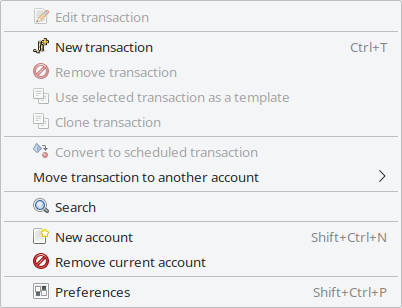
\includegraphics[width=1\textwidth]{image/screenshot/home_menubar_edit}
	\vspace{-15pt}					% space between the floating and the caption below the floating
	\captionsetup{
		type=figure,%				% define "figure" or "table" type, mandatory
		name=Fig.,%					% rename label caption, default="Figure" (or "Table")
		labelsep=newline}			% define the separator between the label and the caption text
	\caption{\menus{Edit} menu}	% \caption is mandatory to reference a figure in lof
	%\vspace{30pt}					% space below the caption
	\label{home_menubar_edit}
\end{minipage}

\begin{itemize}
	\item \menus{Use selected transaction as a template}: allows you to create a new operation from a selected operation, see \vref{transactions-model}, \menus{Selecting a transaction for use as a template}:
	%\menus{Utiliser l'opération sélectionnée comme modèle}: permet de créer une nouvelle opération à partir d'une opération sélectionnée, voir la section \vref{transactions-model}, \menus{Opération sélectionnée comme modèle};
	\item \menus{Clone transaction}: is used to duplicate an existing operation, see section \vref{transactions-duplicate}, \menus{Clone a transaction};
	%\menus{Cloner l'opération}: permet de dupliquer une opération existante, voir la section \vref{transactions-duplicate}, \menus{Clonage d'une opération};
	\item \menus{Convert to scheduled transaction}: see section \vref{transactions-schedule}, \menus{Converting a transaction to a scheduled transaction};
	%\menus{Convertir en opération planifiée}: voir la section \vref{transactions-schedule}, \menus{Conversion d'une opération en opération planifiée};
	\item \menus{Move transaction to another account}: see section \vref{transactions-move}, \menus{Moving a transaction to another account};
	%\menus{Déplacer l'opération vers un autre compte}: voir la section \vref{transactions-move}, \menus{Déplacement d'une opération vers un autre compte};
	\item \menus{Search}: displays the string or amount search box, """see chapter \vref{reportscreation}, \menus{Création d'un état}""";%TODO to modify
	%\menus{Rechercher}: affiche la fenêtre de	recherche d'une chaîne de caractères ou de montants, """voir le chapitre \vref{reportscreation}, \menus{Création d'un état}""";
	\item \menus{New account}: starts the wizard for creating a new account in your Grisbi file (shortcut \keys{Shift+Ctrl+N}), see section \vref{accounts-new}, \menus{Creating a new account};
	%\menus{Nouveau compte}: démarre l'assistant de	création d'un nouveau compte dans votre fichier Grisbi (raccourci-clavier \keys{Maj \shift+Ctrl+N}), voir la section \vref{accounts-new}, \menus{Création d'un nouveau compte};
	\item \menus{Remove current account}: deletes the selected account from your Grisbi file, see section \vref{accounts-delete}, \menus{Removing the current account}:
	%\menus{Supprimer le compte courant}: efface le compte sélectionné de votre fichier Grisbi, voir la section \vref{accounts-delete}, \menus{Suppression d'un compte};
	\item \menus{Preferences}: allows you to configure Grisbi (shortcut \keys{Maj \shift+Ctrl+P}); see the chapter \vref{setup}, \menus{Configuration of Grisbi}.
	%\menus{Préférences}: permet de configurer Grisbi (raccourci-clavier \keys{Maj \shift+Ctrl+P}); voir le chapitre \vref{setup}, \menus{Configuration de Grisbi}.
\end{itemize}

%TODO following
\subsection{\menus{View} menu\label{home-menus-display}}

This menu includes the following functions: 

\begin{itemize}
	 \item \menus{Show transaction form}: 
	 \item \menus{Show reconciles} (shortcut key \key{Alt}\key{R}):
	 \item \menus{Show lines archives} (shortcut key \key{Altl}\key{L}):
	 \item \menus{Show \indexword{closed accounts}}\index{compte !clos}:
	 \item \menus{Show one line per transaction}:
	 \item \menus{Show two lines per transaction}:
	 \item \menus{Show three lines per transaction}:
	 \item \menus{Show four lines per transaction}:
	 \item \menus{Reset the column width}: allows you to reset the columns of the tranaction lists to their original width.
\end{itemize}


\subsection{\menus{Help} menu\label{home-menus-help}}

Most of the choices in this menu give links to websites. In order for these links to work, you must have specified to Grisbi the navigation software (or browser) that you wish to use, in the \menus{Edit - Preferences} (see \vref{setup-general-programs}, \menus{Programmes}). The \menus{Help} menu includes the following choices\footnote{\strong{Translators Note:} A "help us with translation" menu item is mentioned in the French version of the manual but does note appear in the English version of Grisbi at release 1.0}:

\begin{itemize}
	\item \menus{Manual}: opens your browser to the  \enquote{Grisbi User Manual page} (shortcut key  \key{Ctrl}\key{H}):
	\item \menus{Quick start}: opens your browser to the  \enquote{Grisbi Quick Start page}:
%	\item \menus{Traduction}: opens your browser to the \enquote{Translate Grisbi}, to help us to widen the internationalization of Grisbi:
	\item \menus{About Grisbi...}: displays the program information box: you will find details about the version, the link to Grisbi's site, the acknowledgements page (contributors to the project) and the user license:
	\item \menus{Grisbi website}: opens your browser to the \lang{Grisbi}\footnote{\urlGrisbi{}} web site:
	\item \menus{Report a bug}: opens your browser to the \lang{Grisbi Bug Tracker page}\footnote{\urlBugTracker{}} to allow you to report a bug that you have discovered. You can also follow on this page the evolution of the corrections made to the reported bugs;
	\item \menus{Tip of the day}: opens a dialog box that displays a tip of use, different each time Grisbi starts; you can successively display all the tips, and choose whether or not the display of the tip of the day when starting Grisbi. To remove or reactivate the tip of the day, see \vref{setup-display-messages-trick}, \menus{Tip of the day}.
\end{itemize}


\section{Shortcut keys\label{home-shortcuts}}


Keyboard shortcuts make it easy to enter data and navigate through Grisbi's windows, avoiding the need to move and click. By using the ones corresponding to the most common manipulations for you, you improve your \indexword{ergonomics}\index{ergonomie} by limiting the important movements of your arms.
 
Grisbi has a number of keyboard shortcuts, presented here according to different themes (see also  \vref{introduction-manual-conventions}, \menus{Typographical conventions in this manual}).
.

\subsection{Application and files}

\begin{itemize}
	\item New accounts file: \key{Ctrl}\key{N}
	\item Open an account file: \key{Ctrl}\key{O}
	\item Register the account file: \key{Ctrl}\key{S}
	\item Close the account file: \key{Ctrl}\key{W}
	\item Close Grisbi: \key{Ctrl}\key{Q}
\end{itemize}


\subsection{Navigation panel}

\begin{itemize}
	\item Select a tab or account: \key{ Arrow Up}, \key{Arrow Down}, \key{Page Up} ou \key{Page Down}
\end{itemize}

\subsection{List of transactions and scheduled transactions}

\begin{itemize}
	\item Select a transaction: \key{Enter}
	\item Move selection:\key{Arrow Up} ou \key{Arrow Down}
	\item New transaction:  \key{Enter} on empty line, or \key{Ctrl}\key{T}
	\item Modify an transaction: \key{Enter}
	\item Delete an transaction: \key{Delete}:
	\item Select a transaction for a reconciliation:\key{Ctrl}\key{P}
	\item Remove a reconciled transaction: \key{Ctrl}\key{R}
	\item Show or hide archival lines: \key{Altl}\key{L}
\end{itemize}


\subsection{Entry form}

\begin{itemize}
	\item The \key{Enter} is configurable: it can be set to either move in the input form, or to validate the entry
	\item Move to the next field: \key{Tab} (depending on your configuration choice)
	\item Cancel the current entry: \key{Esc}
	\item Accept auto-complete: \key{Tab} or \key{Enter} (depending on your configuration choice)
	\item  Euro symbol: \key{AltGr}\key{e}
\end{itemize}

\subsection{Drop down lists}

\begin{itemize}
	 \item Open a list: \key{Page Down} or \key{Down Arrow}
	 \item Move in the list: \key{Up Arrow}, \key{Down Arrow}, \key{Page Up} or \key{Page Down}
	 \item Validate a choice within a list: \key{Enter}
	 \item Currencies, ??exercises?? and methods of payment:
		\begin{itemize}
			\item open list: \key{Space}: 
			\item move in the list: \key{Up Arrow} or \key{Down Arrow}:
			\item validate the item in the list: \key{Space}.
		\end{itemize}
\end{itemize}


\subsection{Dates entered on the calendar}

\begin{itemize}
	\item Opens a calendar (on the date field): \key{Ctrl}\key{Enter}
	\item Closes the calendar without changing the date: \key{Esc}
	\item Validate the selected date: \key{Enter}
	\item Next or previous day: \key{+} or \key{-}, \key{Right Arrow} or \key{Left Arrow}
	\item Previous or next week: \key{Up Arrow} or \key{Down Arrow}
	\item Previous or next month: \key{Page Up} or \key{Page Down}
	\item First day or last day of the month: \key{Start} or \key{End}
\end{itemize}


\subsection{Dates entered on keyboard }

\begin{itemize}
	\item Next or previous day: \key{+} or \key{-}
	\item Previous or next week: \key{Shift} \key{+} or \key{Majuscule} \key{-}
	\item Previous or next month: \key{Page Up} or \key{Page Down}
	\item Previous or Next Year: \key{Shift} \key{Page Up} or \key{Shift} \key{Page Down}
	\item Validate the selected date \key{Enter}
\end{itemize}


\subsection{Payees, categories, budget allocations, credit simulator, historical data and forecasts}

\begin{itemize}
	\item Move selection: \key{Up Arrow}, \key{Down Arrow}, \key{Page Up} or \key{Page Down}
%Ces raccourcis ne fonctionnent plus:
%	\item afficher les sous-catégories ou sous-imputations budgétaires (sur une catégorie ou une imputation budgétaire): \key{Espace}:
%	\item afficher les opérations des sous-catégories ou sous-imputations budgétaires (sur une sous-catégorie ou une sous-imputation budgétaire): \key{Espace}.
\end{itemize}


\subsection{States and Configuration}

\begin{itemize}
	\item Select another tab: \key{Up Arrow}, \key{Down Arrow}, \key{Page Up}, \key{Page Down}
	\item Navigate between the tab panel and the different options in the settings panel: \key{Tab}, \key{Up Arrow}, \key{Down Arrow}, \key{Left Arrow} and \key{Right Arrow}
\end{itemize}

\subsection{Help}

\begin{itemize}
	\item Open your browser on the Grisbi User Manual page \key{Ctrl}\key{H}
\end{itemize}













